\bmhead{Acknowledgements}
The author thanks the creators of the RAVDESS, CREMA-D, CMU-MOSEI and DEMAND corpora for making their data publicly available for research.

\section*{Declarations}

\bmhead{Funding}
No funding was received for conducting this study.

\bmhead{Competing interests}
The author has no competing interests to declare that are relevant to the content of this article.

\bmhead{Ethics approval and consent to participate}
This study used only the publicly available RAVDESS \citep{livingstone2018} and CREMA-D \citep{cao2014} corpora, which were collected with the informed consent of the participating actors and are distributed for research use, the CMU-MOSEI corpus \citep{zadeh2018}, which consists of videos posted publicly online and is distributed for research, and the DEMAND noise corpus \citep{thiemann2013}, which contains no speech. No new data were collected from human participants.

\bmhead{Data availability}
The RAVDESS corpus is available from Zenodo (\url{https://doi.org/10.5281/zenodo.1188976}) under a CC BY-NC-SA 4.0 licence. CREMA-D is available from \url{https://github.com/CheyneyComputerScience/CREMA-D} under the Open Database License, and DEMAND from Zenodo (\url{https://doi.org/10.5281/zenodo.1227121}). CMU-MOSEI and its labels are available through the CMU Multimodal SDK (\url{https://github.com/CMU-MultiComp-Lab/CMU-MultimodalSDK}); the list of the 2346 selected segments and the rule used to select them are part of the released code.

\bmhead{Code availability}
The feature extraction, experiment and analysis code, together with all result tables, is available at \url{https://github.com/vinhqdang/Artificial-Intelligence-Affective-Computing-and-Video-Analytics-for-Intelligent-Information-Systems}.

\bmhead{Author contributions}
Quang-Vinh Dang conceived and designed the study, performed the analysis and wrote the manuscript.

\begin{appendices}

\section{Additional results}\label{app:extra}

\begin{figure}[ht]
\centering
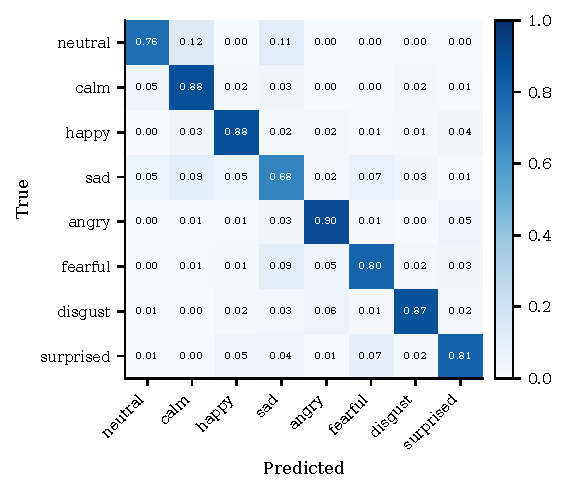
\includegraphics[width=0.55\textwidth]{figures/confusion.pdf}
\caption{Row-normalised confusion matrix of F-all (late fusion of all four models) on held-out actors, clean condition.}\label{fig:confusion}
\end{figure}

\begin{figure}[ht]
\centering
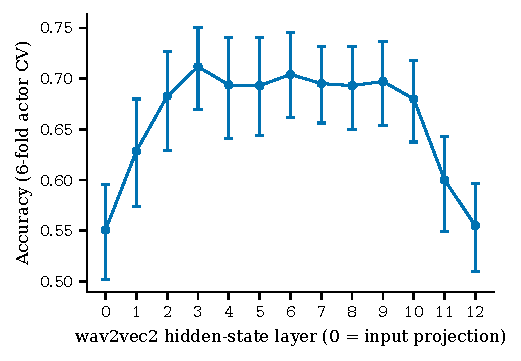
\includegraphics[width=0.55\textwidth]{figures/layer_probe.pdf}
\caption{Subject-independent accuracy of a logistic-regression probe on each single wav2vec~2.0 layer (clean condition, $C=0.1$). The layer-averaged representation used in the artifact reaches 0.721.}\label{fig:layers}
\end{figure}


\begin{table}[ht]
\caption{Share of test clips (\%) whose monitor score exceeds the per-clip P99 threshold, by condition, for monitors fitted on the clean training clips of each fold (mean over folds). Produced by \texttt{diag\_qd\_envelope.py}.}\label{tab:envelope}
\centering\footnotesize
\begin{tabular}{@{}lrrrr@{}}
\toprule
 & \multicolumn{2}{c}{CREMA-D} & \multicolumn{2}{c}{CMU-MOSEI} \\
\cmidrule(lr){2-3}\cmidrule(l){4-5}
Channel and condition & QD & CONTENT & QD & CONTENT \\
\midrule
audio clean & 1.1 & 1.1 & 1.0 & 1.0 \\
audio snr10 & 100.0 & 40.4 & 0.9 & 0.1 \\
audio snr0 & 100.0 & 100.0 & 94.2 & 0.1 \\
audio cafe5 & 94.9 & 4.1 & 0.6 & 0.2 \\
audio street5 & 86.0 & 0.1 & 0.6 & 0.2 \\
\midrule
video clean & 1.1 & 1.5 & 1.2 & 1.5 \\
video compress & 11.8 & 79.3 & 0.4 & 0.6 \\
video lowlight & 86.8 & 16.8 & 0.2 & 1.0 \\
video h264 & 0.9 & 7.5 & 0.5 & 0.9 \\
\botrule
\end{tabular}
\end{table}

\end{appendices}
